% !TEX TS-program = pdflatex
% !TEX encoding = UTF-8 Unicode
%%
%% This is file `sample-sigconf.tex',
%% generated with the docstrip utility.
%%
%% The original source files were:
%%
%% samples.dtx  (with options: `sigconf')
%% 
%% IMPORTANT NOTICE:
%% 
%% For the copyright see the source file.
%% 
%% Any modified versions of this file must be renamed
%% with new filenames distinct from sample-sigconf.tex.
%% 
%% For distribution of the original source see the terms
%% for copying and modification in the file samples.dtx.
%% 
%% This generated file may be distributed as long as the
%% original source files, as listed above, are part of the
%% same distribution. (The sources need not necessarily be
%% in the same archive or directory.)
%%
%%
%% Commands for TeXCount
%TC:macro \cite [option:text,text]
%TC:macro \citep [option:text,text]
%TC:macro \citet [option:text,text]
%TC:envir table 0 1
%TC:envir table* 0 1
%TC:envir tabular [ignore] word
%TC:envir displaymath 0 word
%TC:envir math 0 word
%TC:envir comment 0 0
%%
%%
%% The first command in your LaTeX source must be the \documentclass command.
\documentclass[sigconf]{acmart}
\usepackage{graphicx}

\settopmatter{printacmref=false} % Removes citation information below abstract
\renewcommand\footnotetextcopyrightpermission[1]{} % removes footnote with conference information in first column
%%\pagestyle{plain} % removes running headers
\thispagestyle{empty}
%%
%% \BibTeX command to typeset BibTeX logo in the docs
\AtBeginDocument{%
    \providecommand\BibTeX{{%
        \normalfont B\kern-0.5em{\scshape i\kern-0.25em b}\kern-0.8em\TeX}}}

%% Rights management information.  This information is sent to you
%% when you complete the rights form.  These commands have SAMPLE
%% values in them; it is your responsibility as an author to replace
%% the commands and values with those provided to you when you
%% complete the rights form.
\setcopyright{none}
\copyrightyear{}
\acmYear{}
\acmDOI{}

%% These commands are for a PROCEEDINGS abstract or paper.
\acmConference[Computer Science]{}{University of Salerno}{UNISA}
\acmBooktitle{Real time Alexa packets profiling analysis}
\acmPrice{}
\acmISBN{}


%%
%% Submission ID.
%% Use this when submitting an article to a sponsored event. You'll
%% receive a unique submission ID from the organizers
%% of the event, and this ID should be used as the parameter to this command.
%%\acmSubmissionID{123-A56-BU3}

%%
%% The majority of ACM publications use numbered citations and
%% references.  The command \citestyle{authoryear} switches to the
%% "author year" style.
%%
%% If you are preparing content for an event
%% sponsored by ACM SIGGRAPH, you must use the "author year" style of
%% citations and references.
%% Uncommenting
%% the next command will enable that style.
%%\citestyle{acmauthoryear}

%%
%% end of the preamble, start of the body of the document source.
\begin{document}

%%
%% The "title" command has an optional parameter,
%% allowing the author to define a "short title" to be used in page headers.
    \title{Real time Alexa packets profiling analysis}


%%
%% The "author" command and its associated commands are used to define
%% the authors and their affiliations.
%% Of note is the shared affiliation of the first two authors, and the
%% "authornote" and "authornotemark" commands
%% used to denote shared contribution to the research.
    \author{Giuseppe Polese}
    \orcid{0000-0002-8496-2658}
    \email{gpolese@unisa.it}
    \affiliation{%
        \institution{Universit\'a degli studi di Salerno}
        \streetaddress{}
        \city{Salerno}
        \state{}
        \country{Italy}
        \postcode{}
    }

    \author{Bernardo Breve}
    \orcid{0000-0002-3898-7512}
    \email{bbreve@unisa.it}
    \author{Stefano Cirillo}
    \orcid{0000-0003-0201-2753}
    \email{scirillo@unisa.it}
    \affiliation{%
        \institution{Universit\'a degli studi di Salerno}
        \streetaddress{}
        \city{Salerno}
        \state{}
        \country{Italy}
        \postcode{}
    }

    \author{Biagio Boi}
    \email{b.boi@studenti.unisa.it}
    \affiliation{%
        \institution{Universit\'a degli studi di Salerno}
        \streetaddress{}
        \city{Salerno}
        \state{}
        \country{Italy}
        \postcode{}
    }

%%
%% The abstract is a short summary of the work to be presented in the
%% article.
    \begin{abstract}
        Nowadays, the introduction of home virtual assistents like Alexa Echo or Google Home became a practice, just considering that over 27\% of families owns one.

        It's obvious that those devices simplified the life by creating a smart house with few money; but what's the impact these devices have on people privacy?
        There are a lot of cases in the United States in which the judge asked to Amazon to provide the recording done by the Echo Dot in order to find helpful
        evidences for the case; so, the question is: "It's possible to prevent the sending of sensible informations to the servers when the weak word is not pronunced?"

        In this project we will profile each packet exchanged between the Alexa Echo and the Server in order to classify the nature of the packets and consequentially we will use a machine learning model to discover when the Echo Dot is sending an inappropriate packet.
    \end{abstract}

%%
%% Keywords. The author(s) should pick words that accurately describe
%% the work being presented. Separate the keywords with commas.
    \keywords{data analytics, alexa, packets profiling}

%% A "teaser" image appears between the author and affiliation
%% information and the body of the document, and typically spans the
%% page.

    \begin{teaserfigure}
        \rule{\linewidth}{1mm}
%%  \includegraphics[width=\textwidth]{sampleteaser}
%%  \caption{Insert text here}
%%  \Description{insert description here}
%%  \label{fig:teaser}
    \end{teaserfigure}

%%
%% This command processes the author and affiliation and title
%% information and builds the first part of the formatted document.
    \maketitle


    \section{Introduction}
    TODO


    \section{Alexa architecture \& security}
    The Alexa architecture isn't really easy to explain, we will resume just the keypoint in order to better understand the main functionalities for our purpose.
    \begin{enumerate}
        \item Alexa is always in listening waiting for the wake word to be pronunced to start the recording of the voice;
        \item From the weak word, till the end of commands, Alexa will record the speech and partially sends it to Alexa Voice Service, that can be considered as the brain of Alexa;
        \item Alexa Voice Service will process the audio using Natural Language Processing and Natural Language Understanding in order to retrieve a response for the given request.
        \begin{enumerate}
            \item Natural Language Processing (NLP) improve the Word Segmentation that separate a chunk of continuous text into separate words.
            \item Natural Language Understanding (NLU) is a subtopic of NLP and uses the AI to map text to the meaning\cite{NLU} in order to understand the speech and the request.
        \end{enumerate}
        \item Depending on the sent command, the Voice Service will take an action (turn on the light) or send the information back to the device and Alexa may speech.
    \end{enumerate}


    \section{State of Art}


    \section{Alexa flow of communication}
    Describe here the entire flow of communication


    \section{Packets analysis}
    In order to create a good dataset we will classify the packets sent by the Echo.
    In particular is possible to classify the type of packet by looking at flags, packet size and protocol used.
    There are different types of packet that will later be included in the dataset as classes:
    \begin{enumerate}
        \item \textbf{handshake}: At the beginning of each new SSL/TLS communication between the Echo and the Server there are different packets exchanged in order to establish a secure communication.
        These packets can be easily identified by the protocol used for the communication (TLS) and by checking the flags related to the content of the message, in particular, the possible flags are:
        \begin{enumerate}
            \item Change Cipher (20).
            \item Server Hello - Show Certificate - Encrypted Message (21).
            \item Alert (22).
        \end{enumerate}
        Echo changes communication Server very frequently, about each 2 minutes.
        \item \textbf{syn}: Two packets with fixed length are sent from the device in a fixed interval, for this reason we believe that these are synchronization packets.
        These packets may be sent to guarantee the synchronization with the Amazon Alexa application and with the Amazon servers.
        There are two possible synchronization packets:
        \begin{enumerate}
            \item A packet of 100 byte is sent each 30 seconds (30002 milliseconds)
            \item A packet of 99 byte is sent each 90 seconds (90820 milliseconds)
        \end{enumerate}
        The communication always happens using SSL/TLS, so it's impossible to decrypt the content of these message and confirm that is securely a synchronization packet.
        \item \textbf{ack}: These are the classical packets used to confirm that the received packets are valid and successfully received.
        \item \textbf{retransmit}: These packets are used to retransmit the data that didn't received an ack, usually this happens when the Echo try to communicate with other Amazon devices (Fire Stick for ex.) but doesn't receive response.
        \item \textbf{app\_data}: These packets are relative to the normal communication of the Echo and can be easily recognized since the communication happens over TLS/SSL protocol and by checking the flag of the considered packet that is equal to 23.
        In particular, we will include in this class all the communication packets that include also recording of voice occurred during the conversation between the Echo and the final costumer.
        \item \textbf{not\_relevant}: We will include in this category all packets that don't match any of the other categories, and are not relevant for our study.
    \end{enumerate}
    It's import to underline that the packets classified as app\_data may include both authorized and not authorized packets.
    The unauthorized packets include all those packets sent in a context in which no application date should be sent to the Server by considering the environmental variables (no wake word pronounced) and hardware aspects (microphone muted by pressing the relative button); for this reason is important to introduce some features related to these aspects.
    The aim is to distinguish three kind of packets:
    \begin{itemize}
        \item \textbf{not\_justified}: packets sent to the Server in a context in which the Echo is unable to send these data by considering the hardware aspects.
        \item \textbf{justified}: packets sent to the Server without any interaction between the Echo and the Customer, but the Echo is able to record.
        \item \textbf{expected}: packets sent to the Server since an interaction between the Echo and the Customer happened.
    \end{itemize}
    Clearly, the only allowed packets are those classified as "Expected".


    \section{Dataset}
    In order to create a valid and well-distributed dataset we analyzed the behavior of the Echo Dot in different context, in particular by considering different cases:
    \begin{enumerate}
        \item \textbf{Microphone mute}: when the hardware button is pressed and the device should be unable to send application data to the server.
        \begin{figure}[h!]
            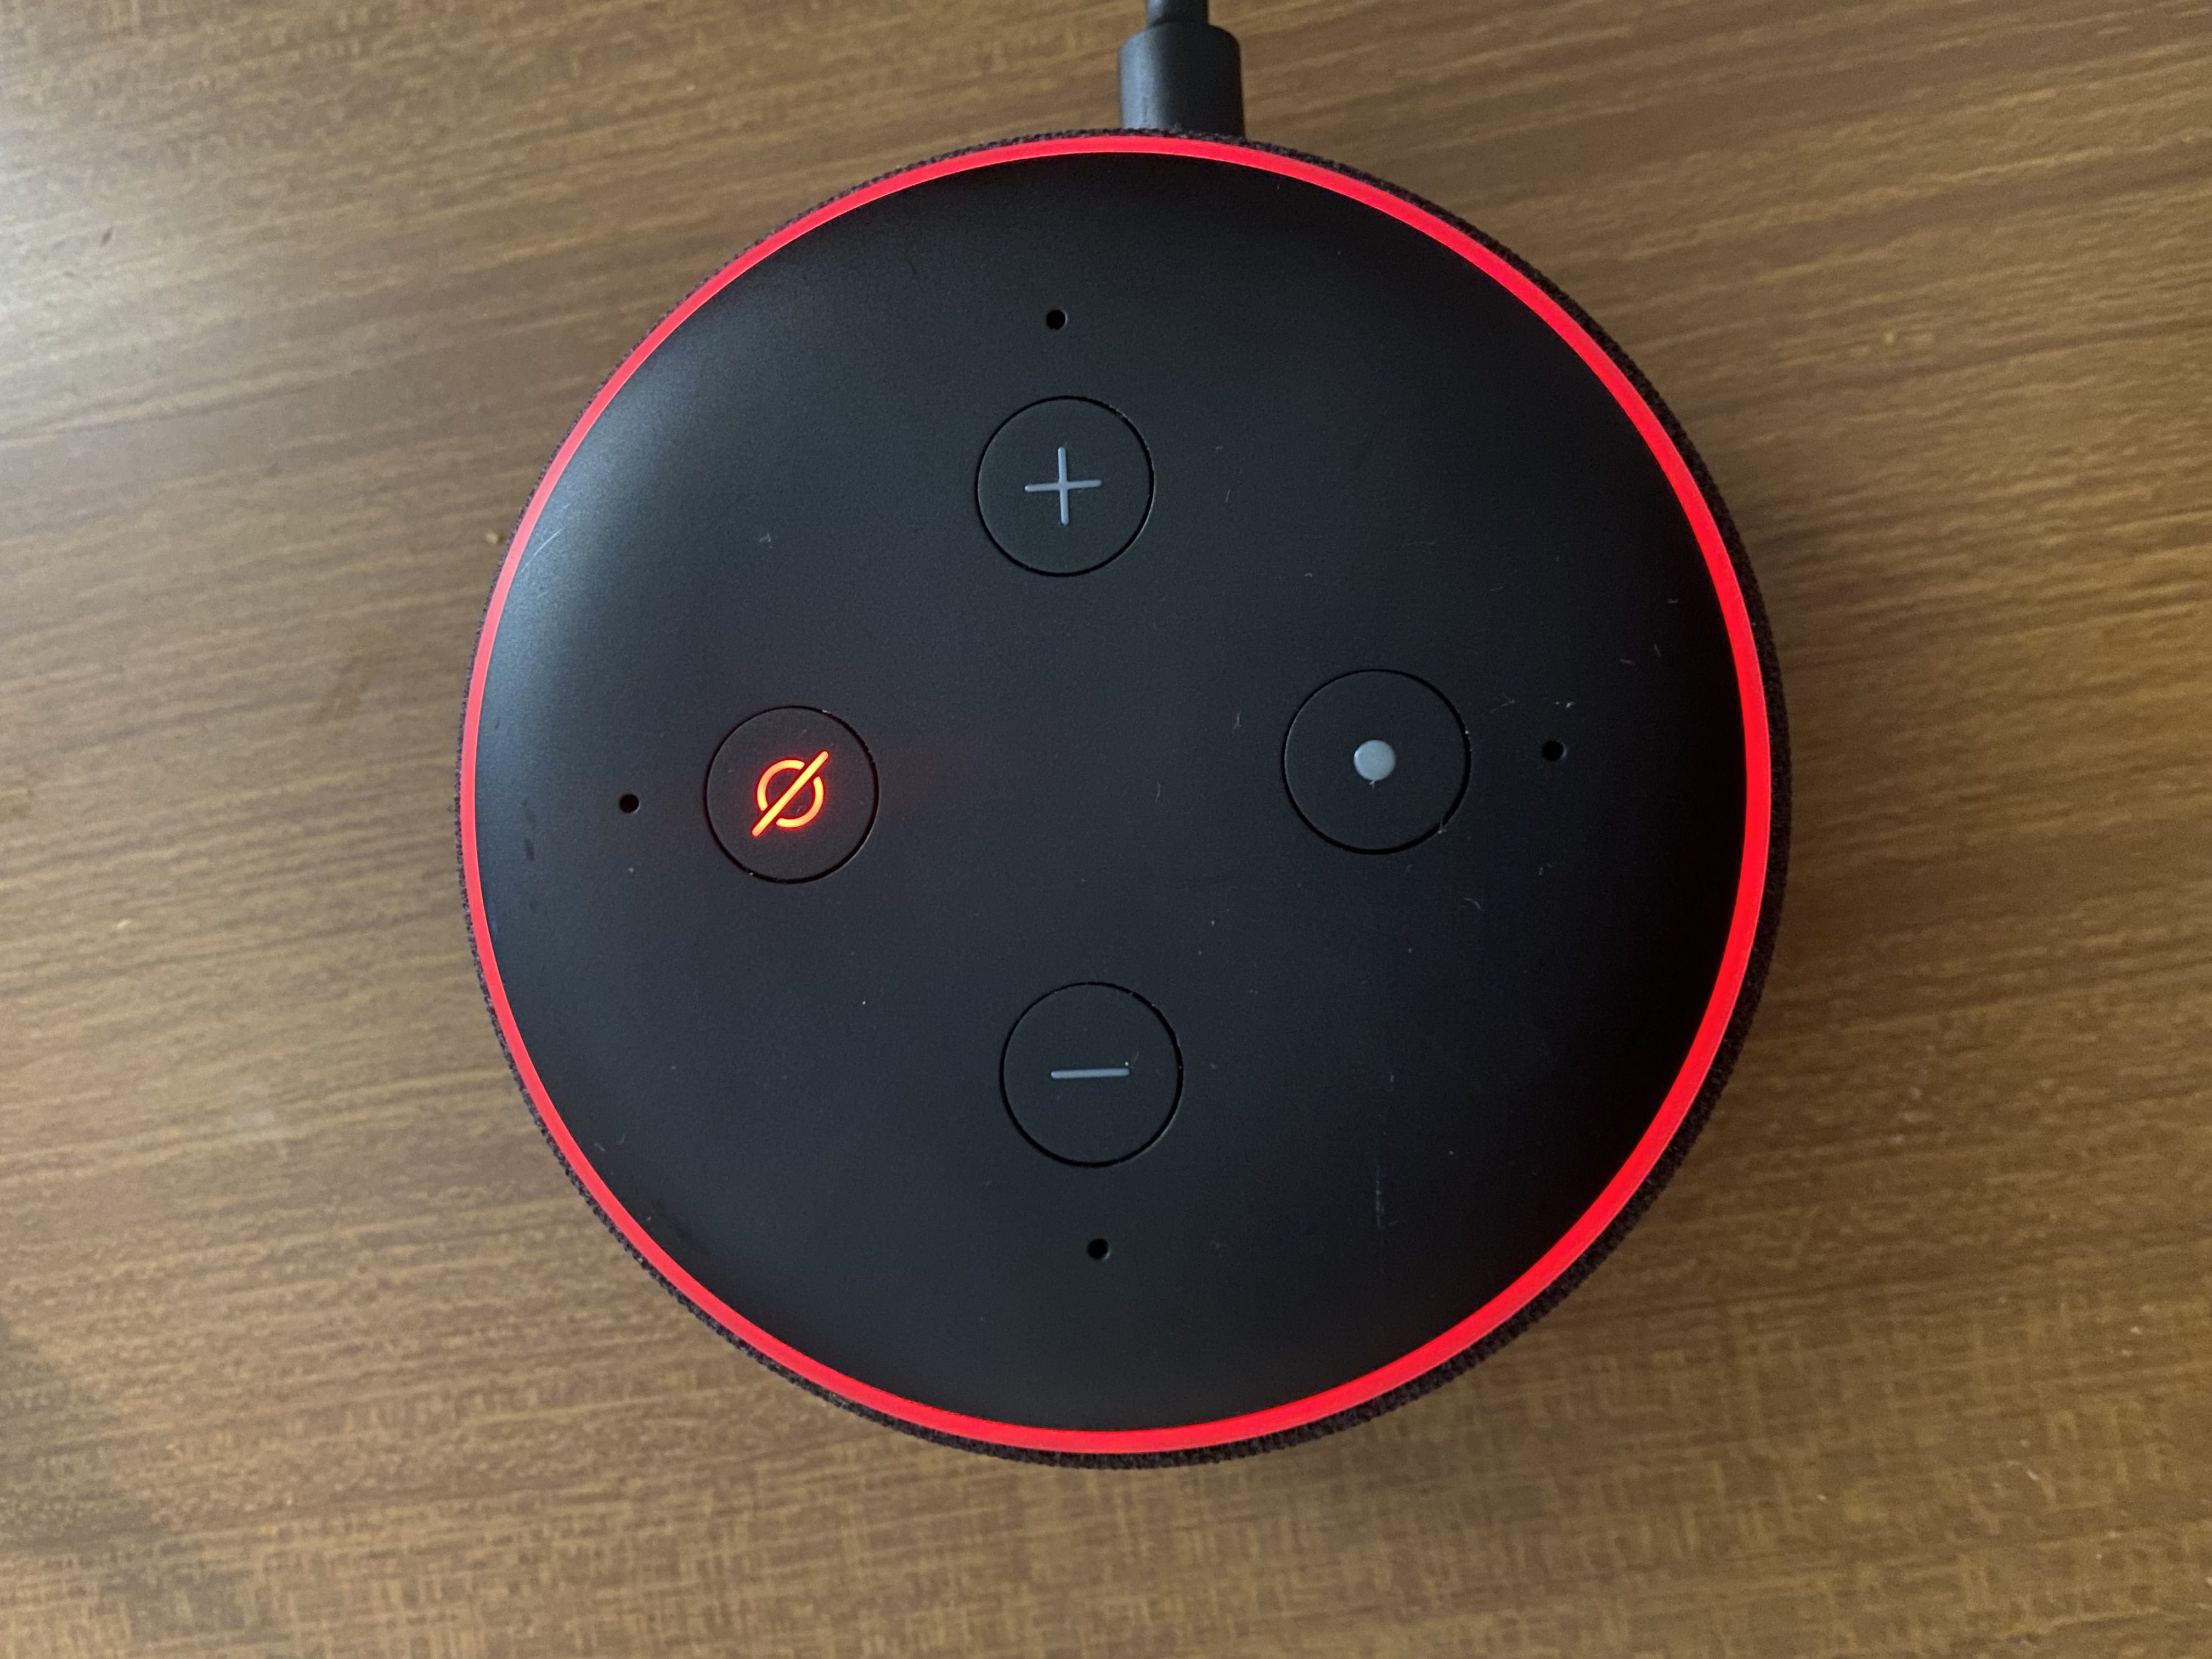
\includegraphics[width=\linewidth]{img/alexa_red.jpg}
            \caption{Echo Dot when the disable microphone button has been pressed.}
            \label{fig:Alexa_red_led}
        \end{figure}
        \item \textbf{No wake word pronounced}: when the device is able to listen the voice but shouldn't send to the Server any packets of application data.
        \item \textbf{Normal stream of data}: when a communication happens.
        It may include different questions or requests, for example:
        \begin{enumerate}
            \item How is the weather today?
            \item When does Liverpool play?
            \item Add water to the cart.
        \end{enumerate}
        All these questions or requests expect a response from the Server, so a huge amount of ack will be sent from the device.
        \item \textbf{Stream of data}: when the user request for a song and the Echo Dot start to stream it.
    \end{enumerate}


    \section{Machine learning}
    TODO


    \section{Conclusions}
    TODO

    \bibliographystyle{ACM-Reference-Format}
    \bibliography{biblio_ref}

\end{document}
\endinput
%%
%% End of file `sample-sigconf.tex'.
